\label{paper_prototype} \chnote{hører til i design?}
A good starting point when designing objects is to prototype the
designs. An easy and inexpensive method of prototyping is paper
prototyping. The following section presents these initial prototypes
to give an overview of how the final software could look like.

\begin{figure}[H]
  \centering
  \subfloat[Listing of nearby venues available.]{
    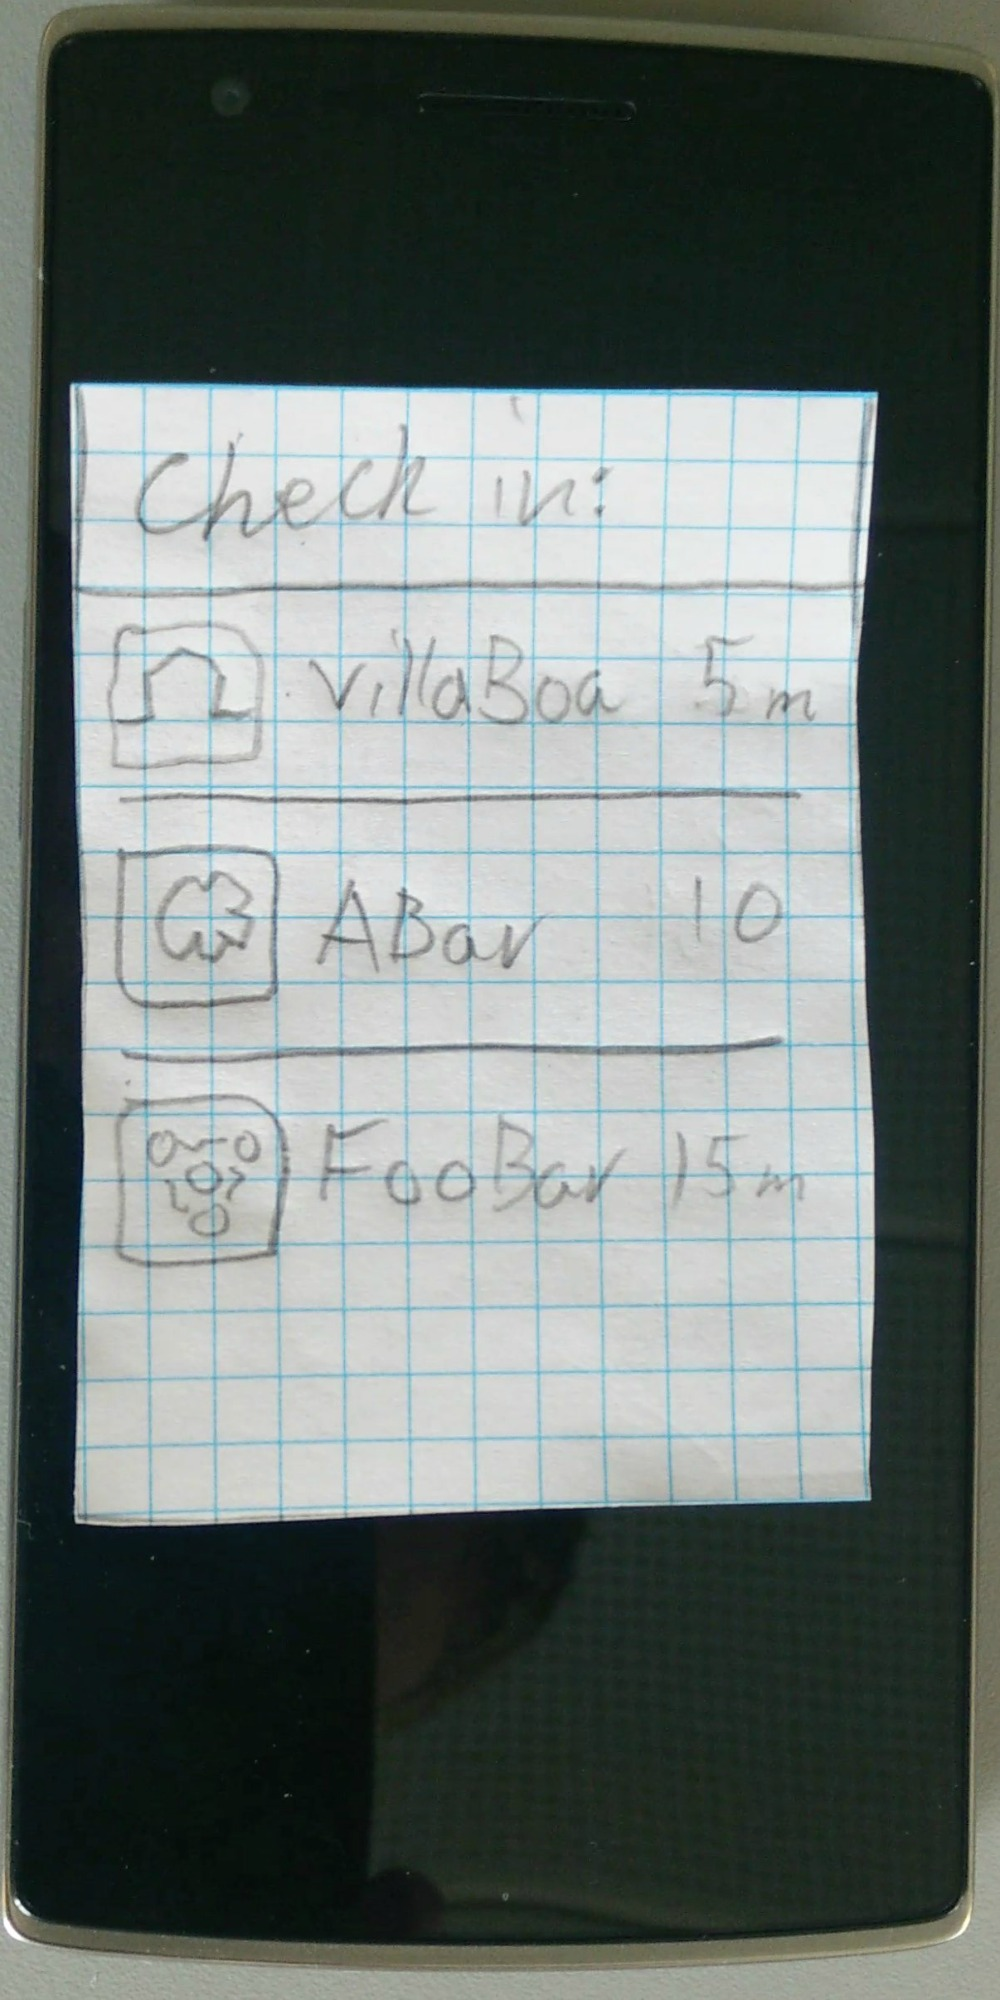
\includegraphics[width=0.3\textwidth]{paperPrototypeCheckin}
    \label{fig:paper_prototype_check_in}
  }
  \subfloat[Interaction with the venue list.]{
    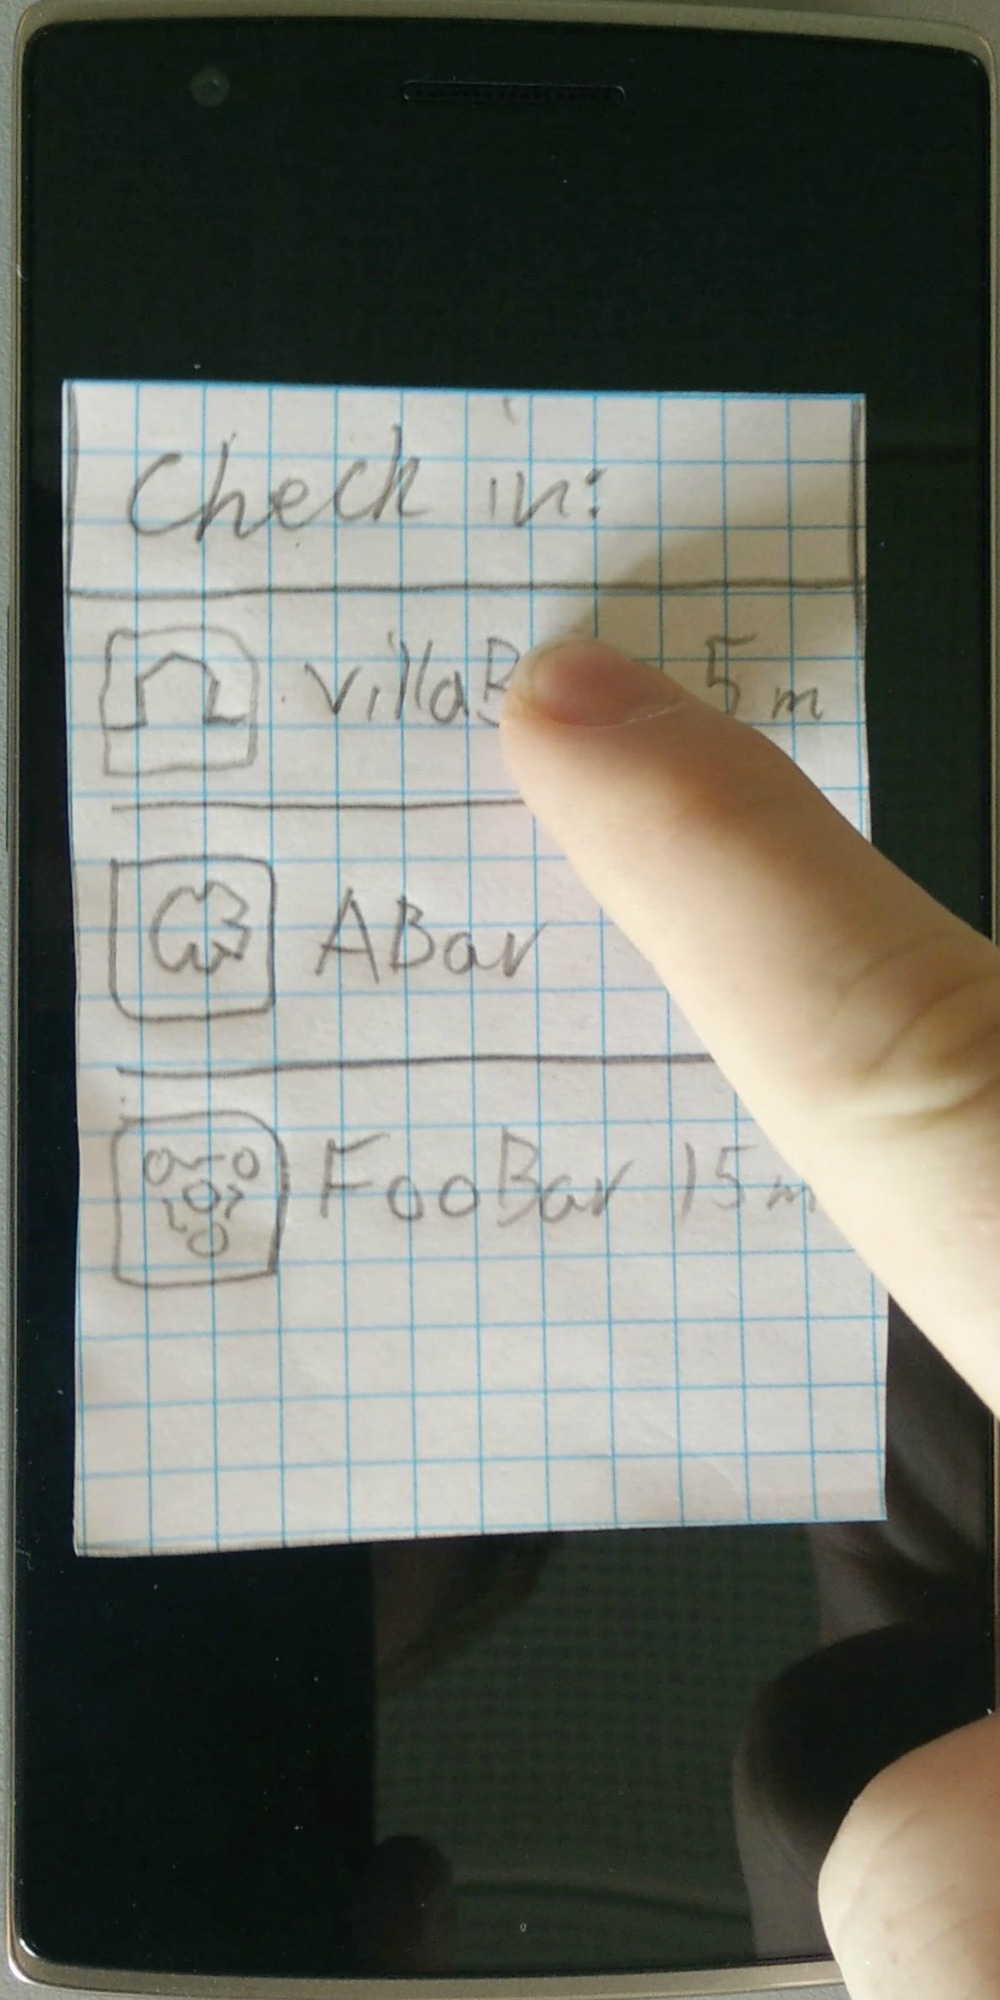
\includegraphics[width=0.3\textwidth]{paperPrototypeCheckinInteraction}
    \label{fig:paper_prototype_check_in_interaction}
  }
  \caption{Check-in screen and interaction with it.}
\end{figure}

One of the first screens presented to the user of the client
application is a check-in screen listing nearby venues using
openPlaylist. See \cref{fig:paper_prototype_check_in}. To select a
venue, one has to press the list item as seen in \cref{fig:paper_prototype_check_in_interaction}.

\begin{figure}[H]
  \centering
  \subfloat[Main screen presenting an interactive playlist.]{
    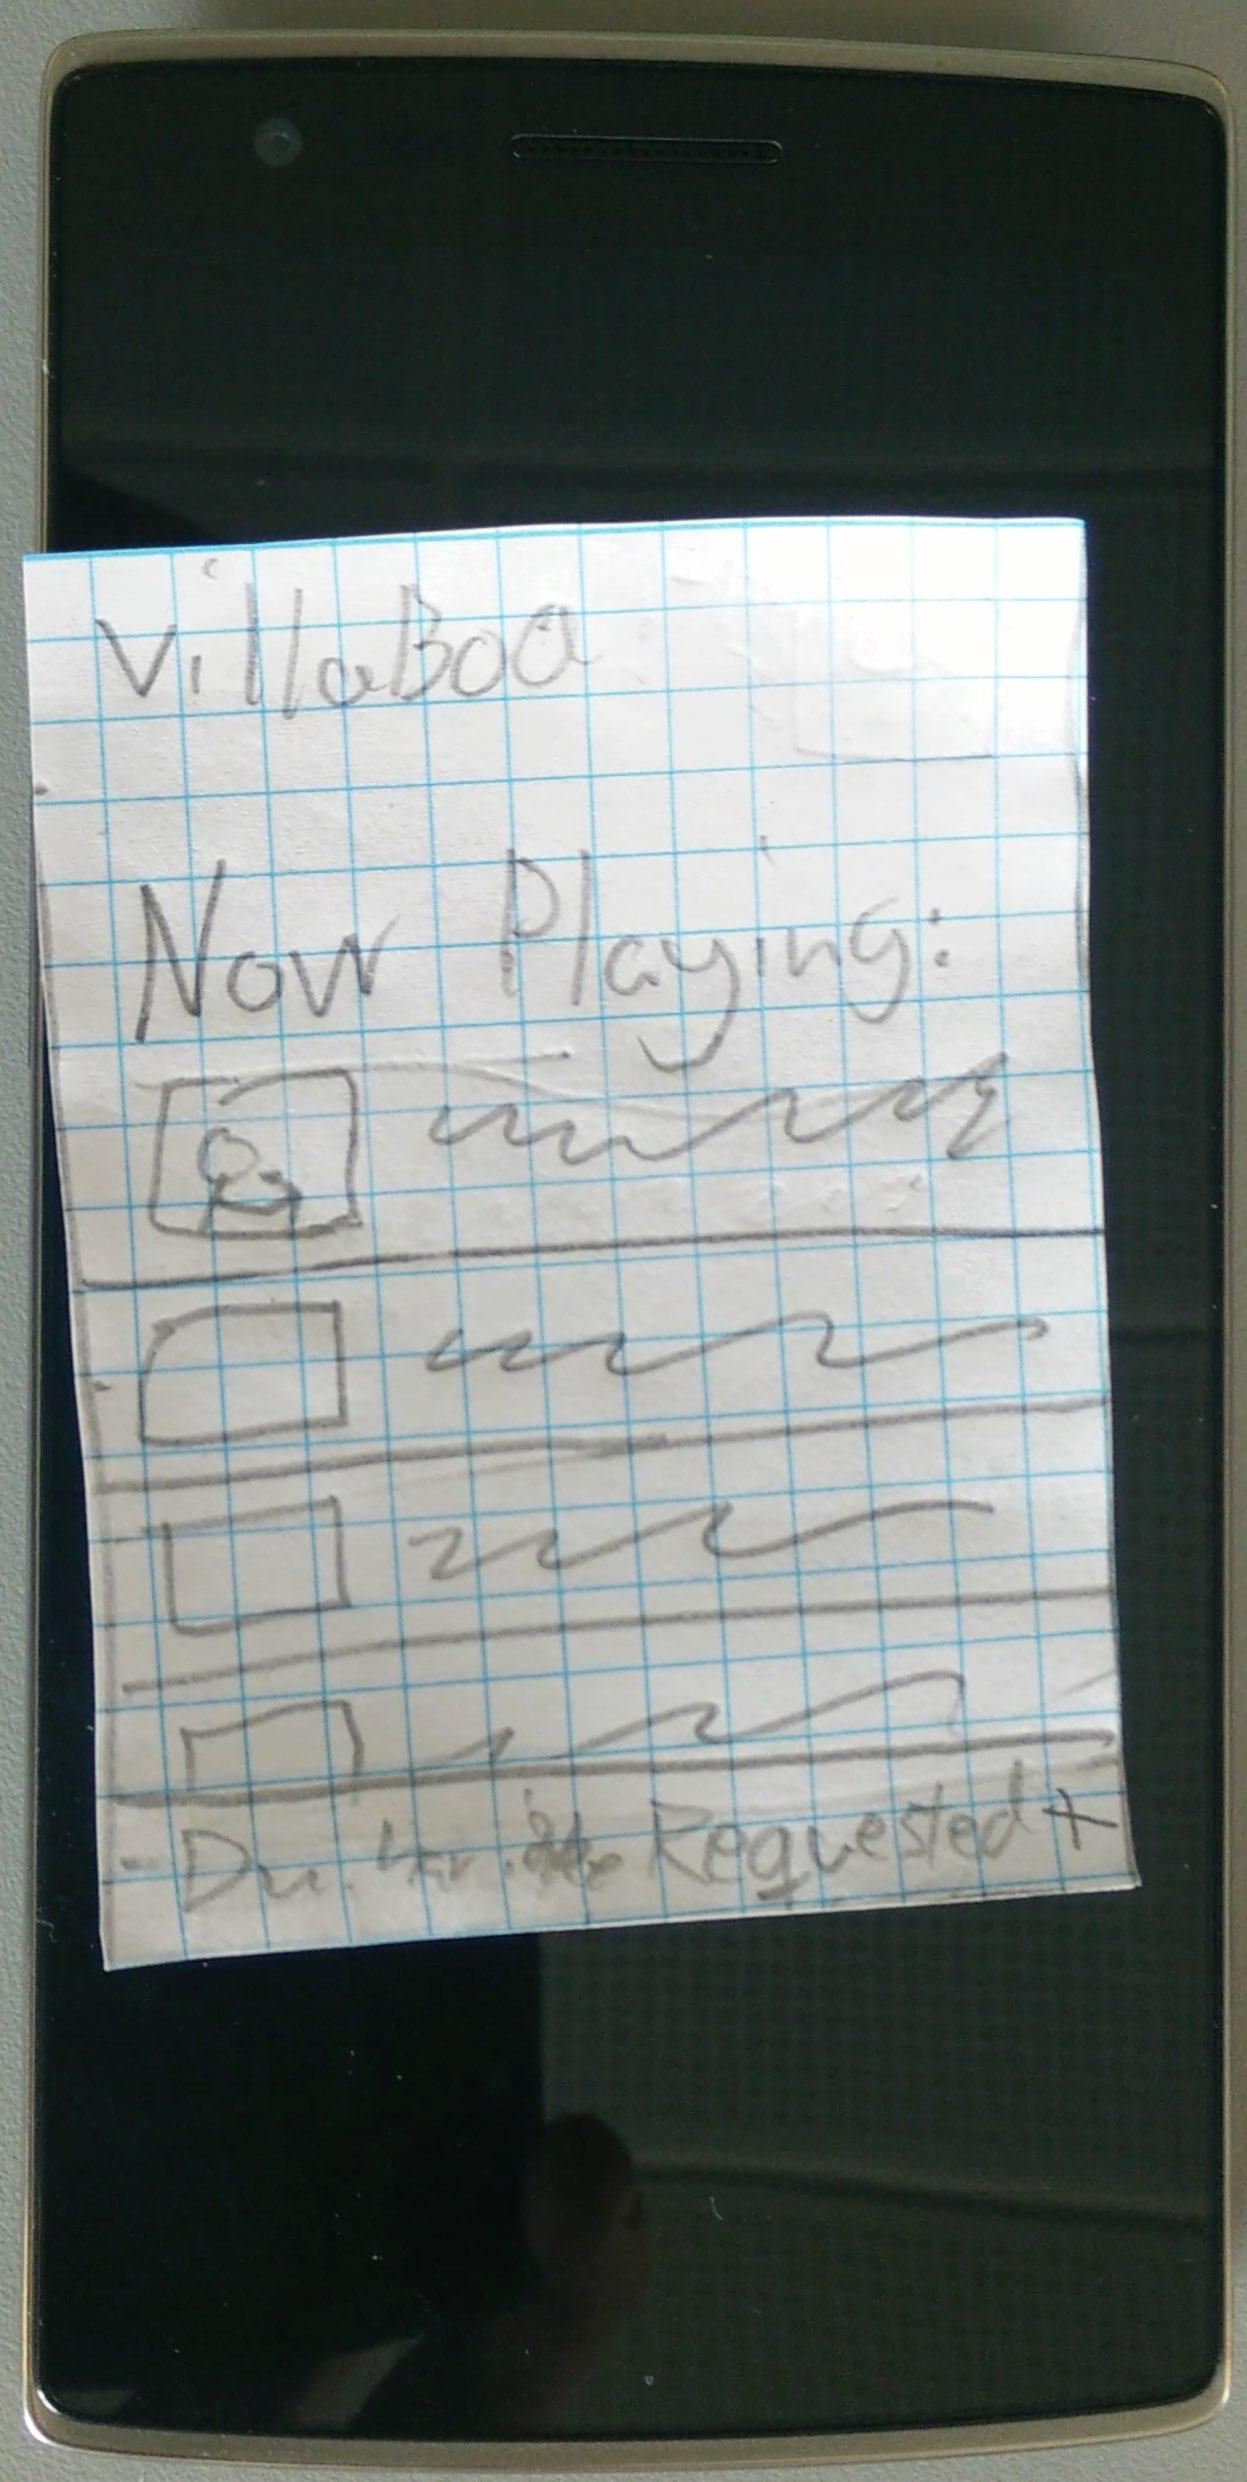
\includegraphics[width=0.33\textwidth]{paperPrototypePlaylist}
    \label{fig:paper_prototype_playlist}

                  }
  \subfloat[Interaction between the playlist and the user.]{
    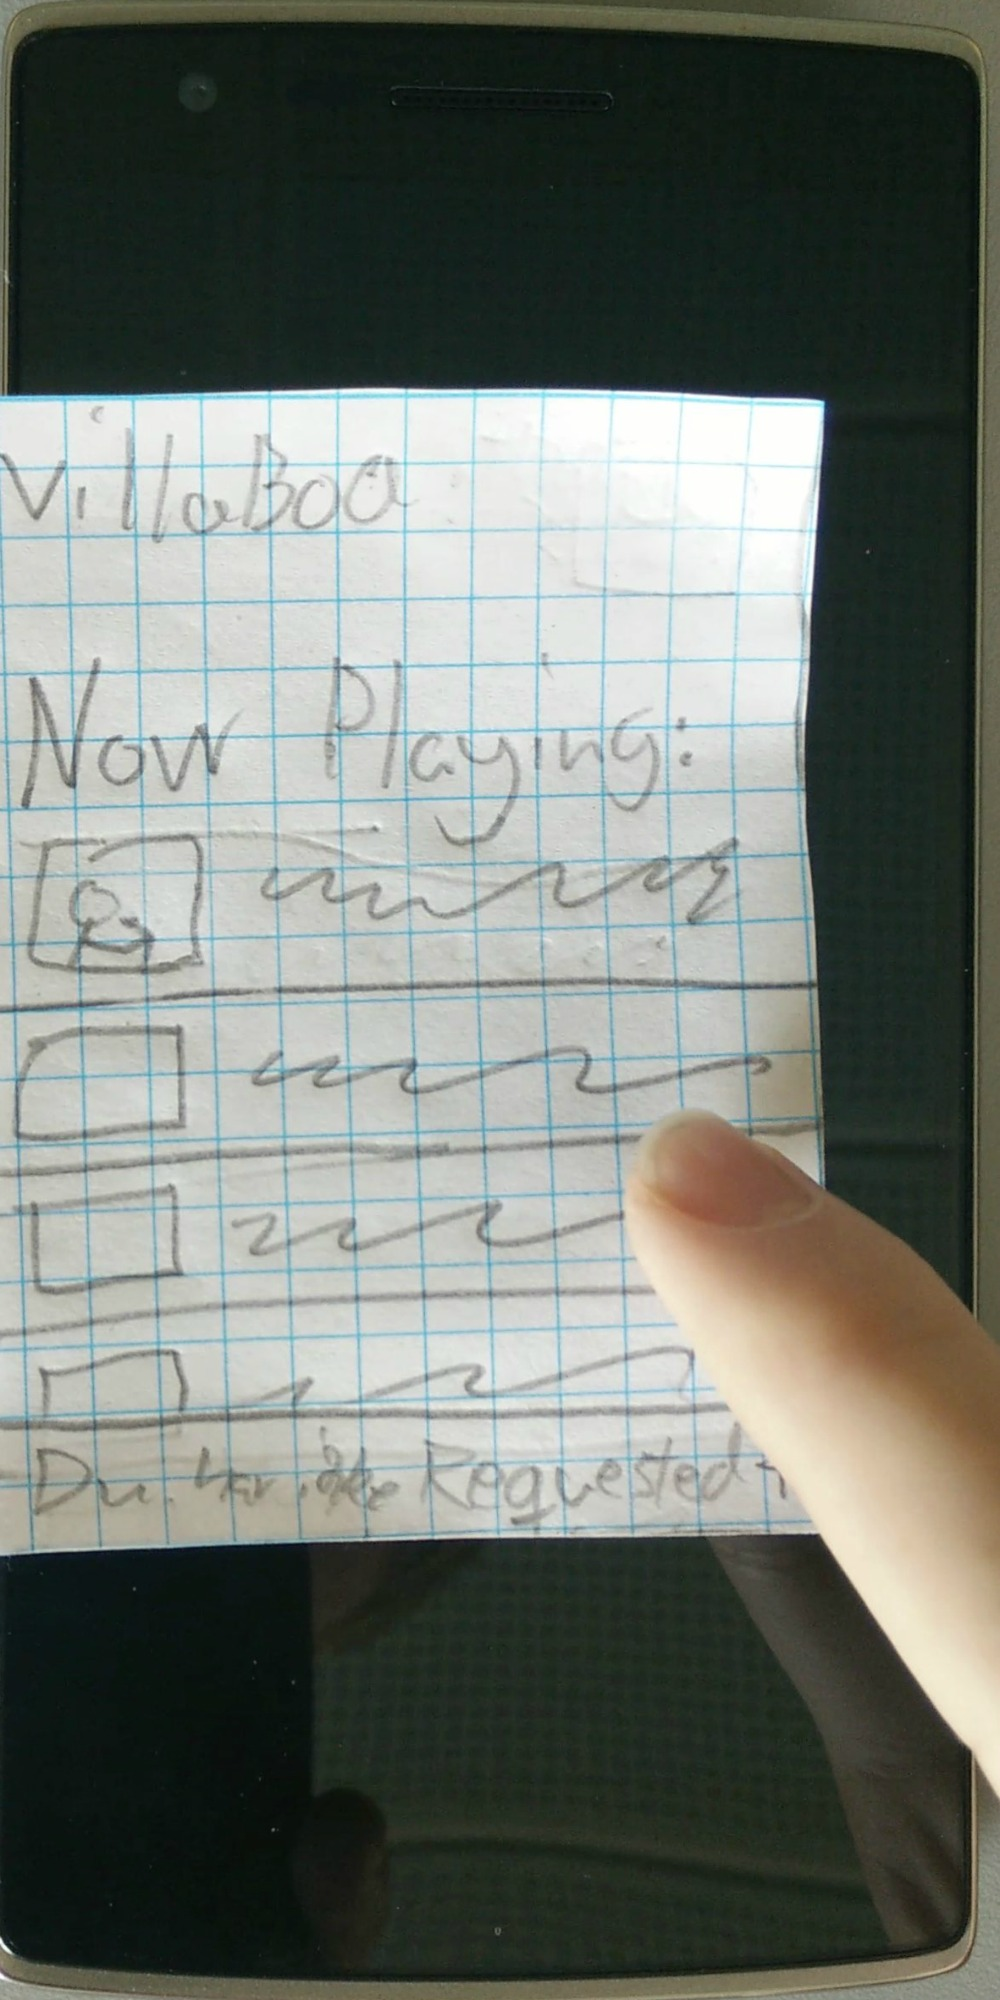
\includegraphics[width=0.33\textwidth]{paperPrototypeVoteInteraction}
    \label{fig:paper_prototype_playlist_interaction}
                  }
  \subfloat[Feedback from the application from a up-vote action.]{
    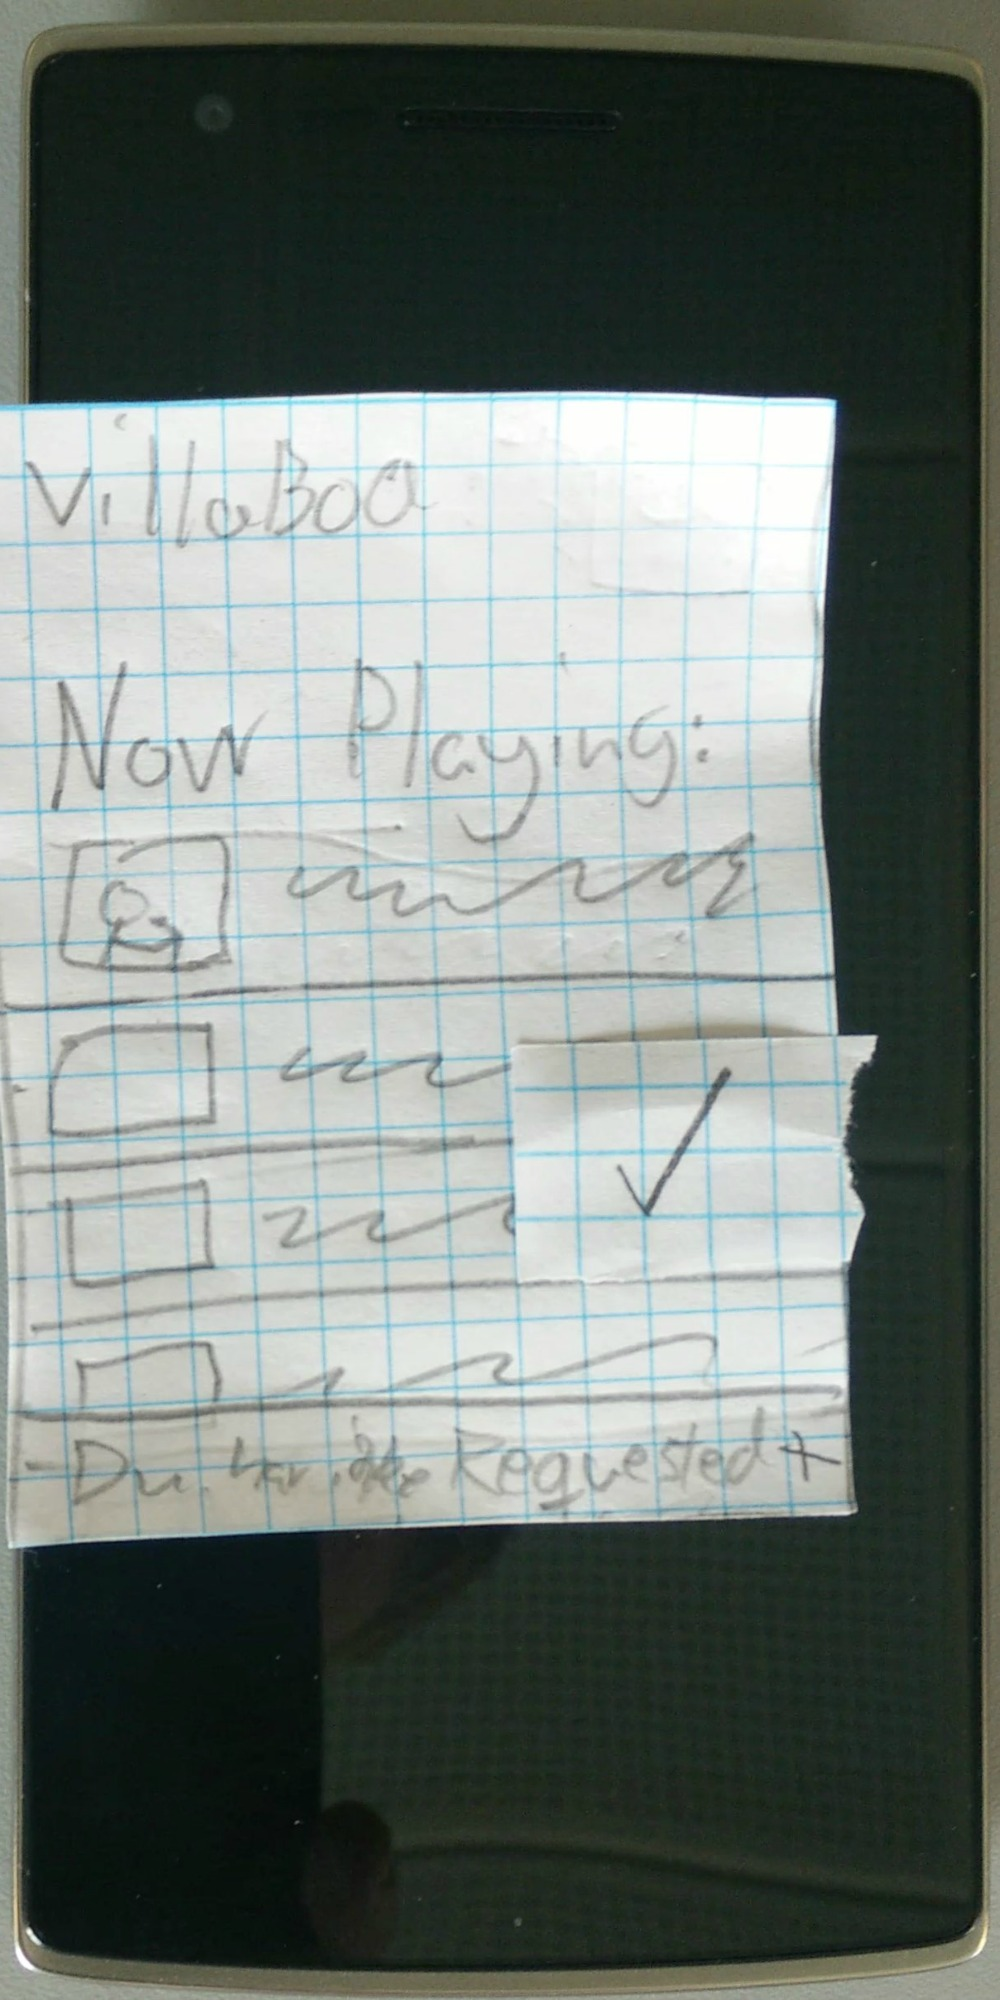
\includegraphics[width=0.33\textwidth]{paperPrototypeVoteFeedback}
    \label{fig:paper_prototype_playlist_feedback}
                  }
  \caption{Voting on a track already on the playlist.}
\end{figure}

Once checked-in to a venue, the user is presented with the playlist of
the venue. See \cref{fig:paper_prototype_playlist}. It is now possible
to influence the playlist, i.e. vote for a track. This
interaction and the corresponding feedback from the system is showcased in
\cref{fig:paper_prototype_playlist_interaction,fig:paper_prototype_playlist_feedback}.

\begin{figure}[H]
  \centering
  \subfloat[Screen displaying search results for a track.]{
    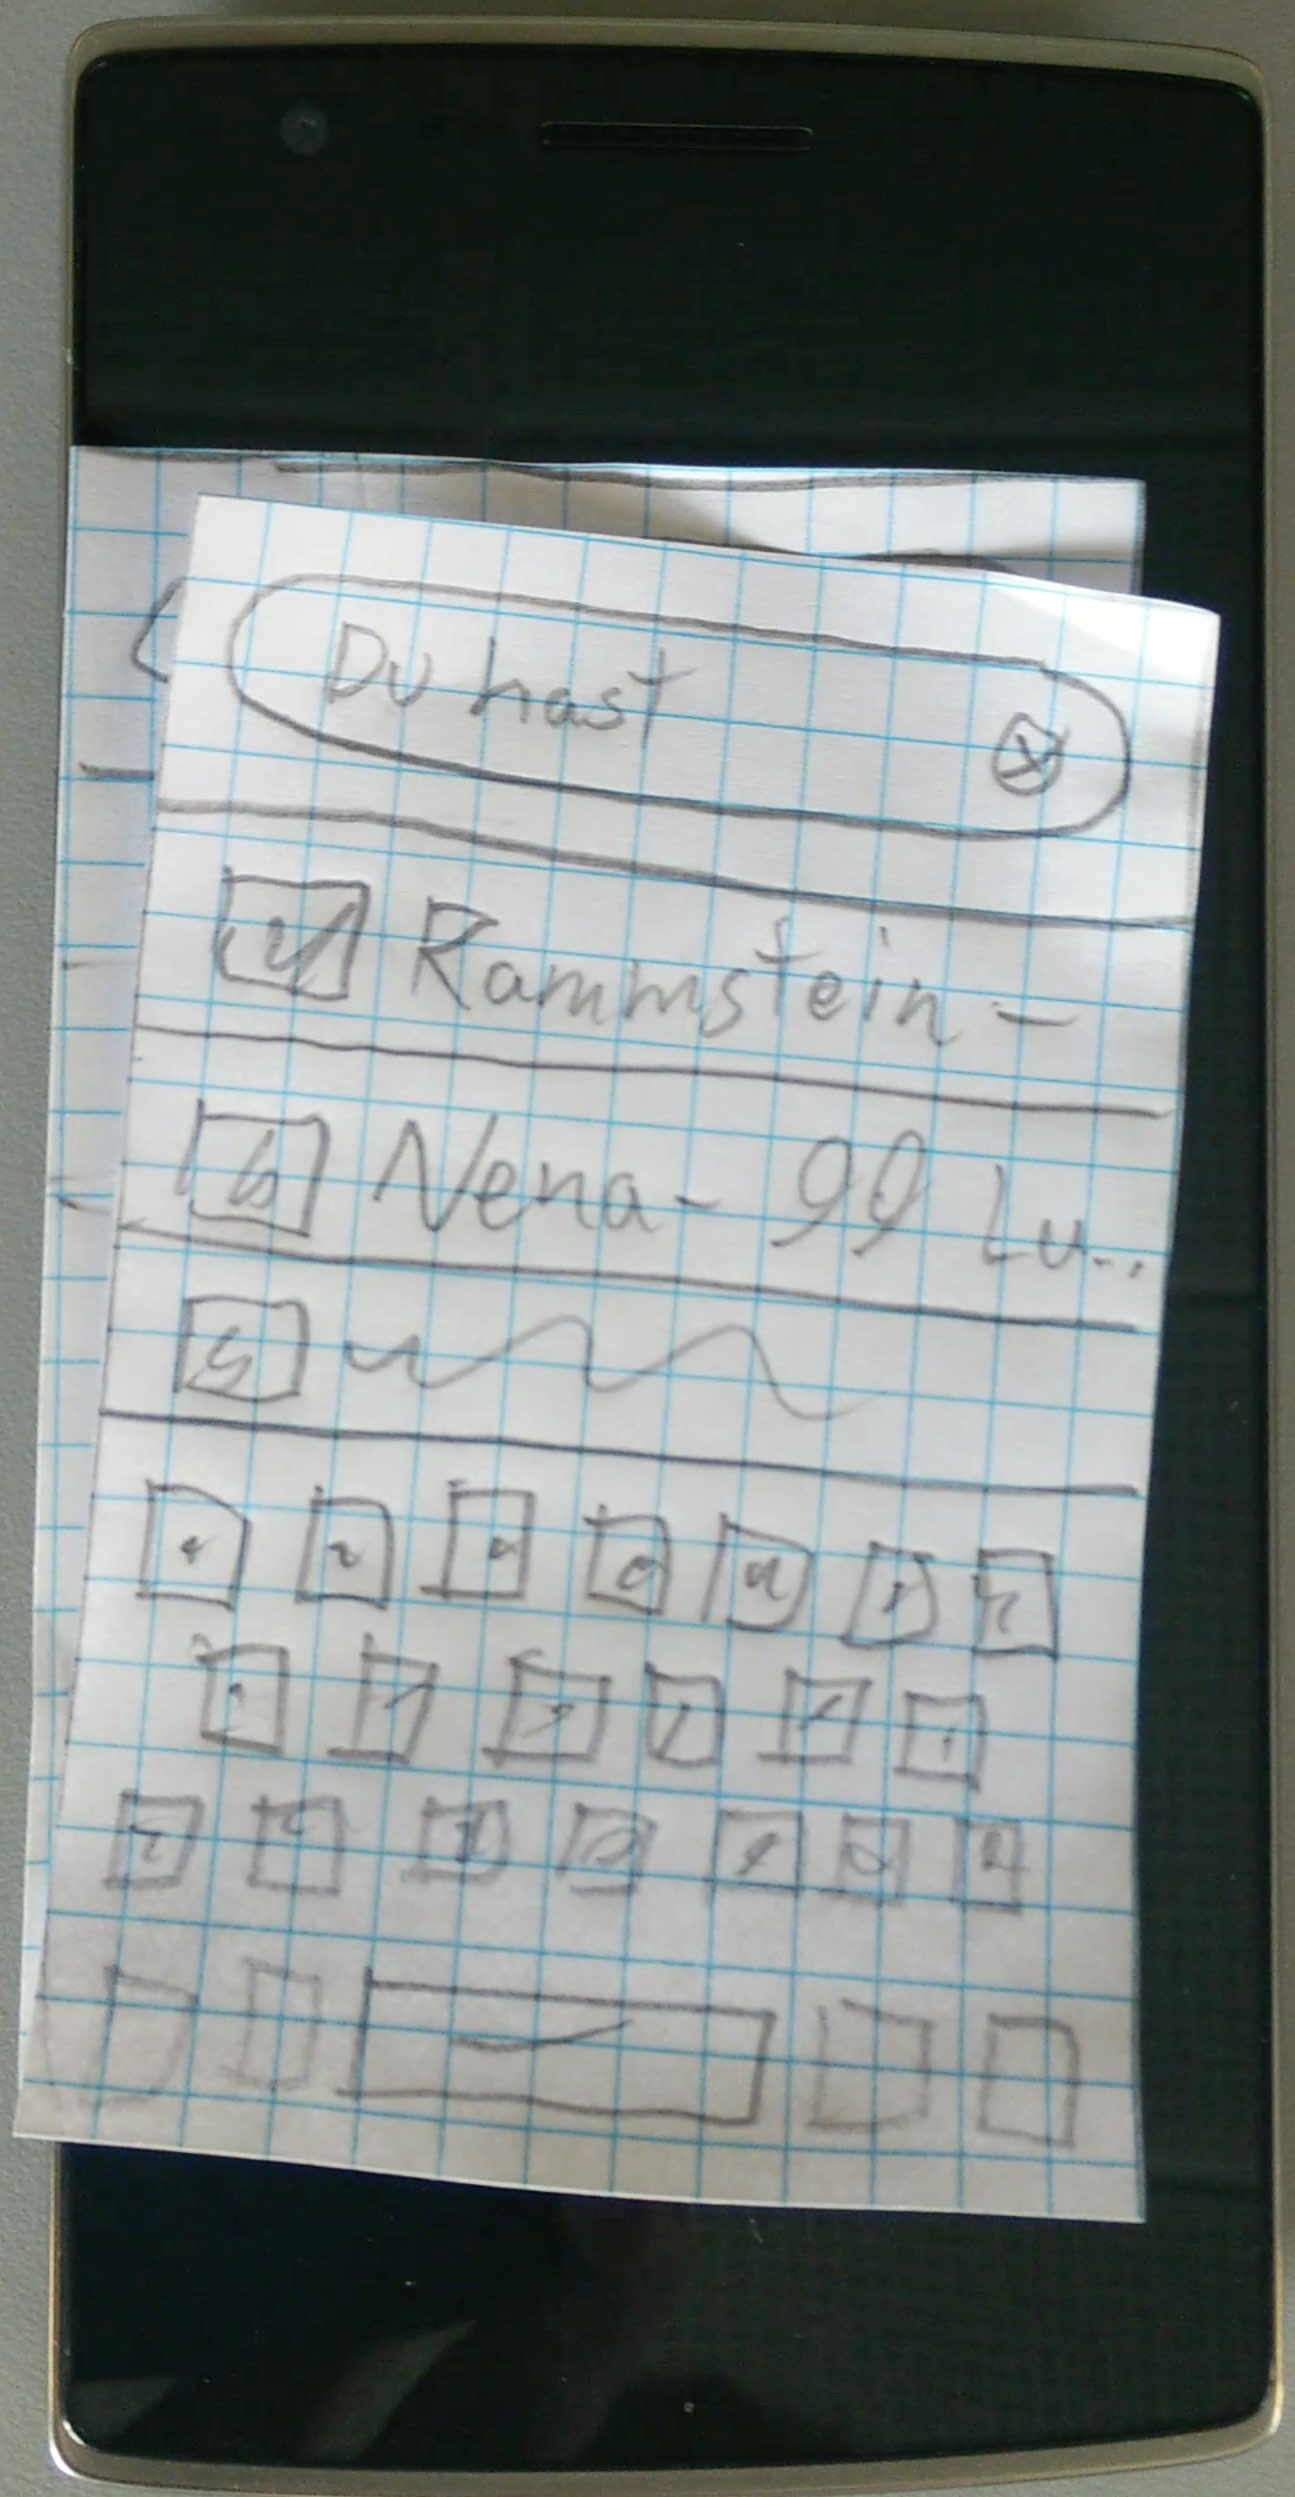
\includegraphics[width=0.33\textwidth]{paperPrototypeAddTrack}
    \label{fig:paper_prototype_add_track}

                  }
  \subfloat[Adding a track to a playlist.]{
    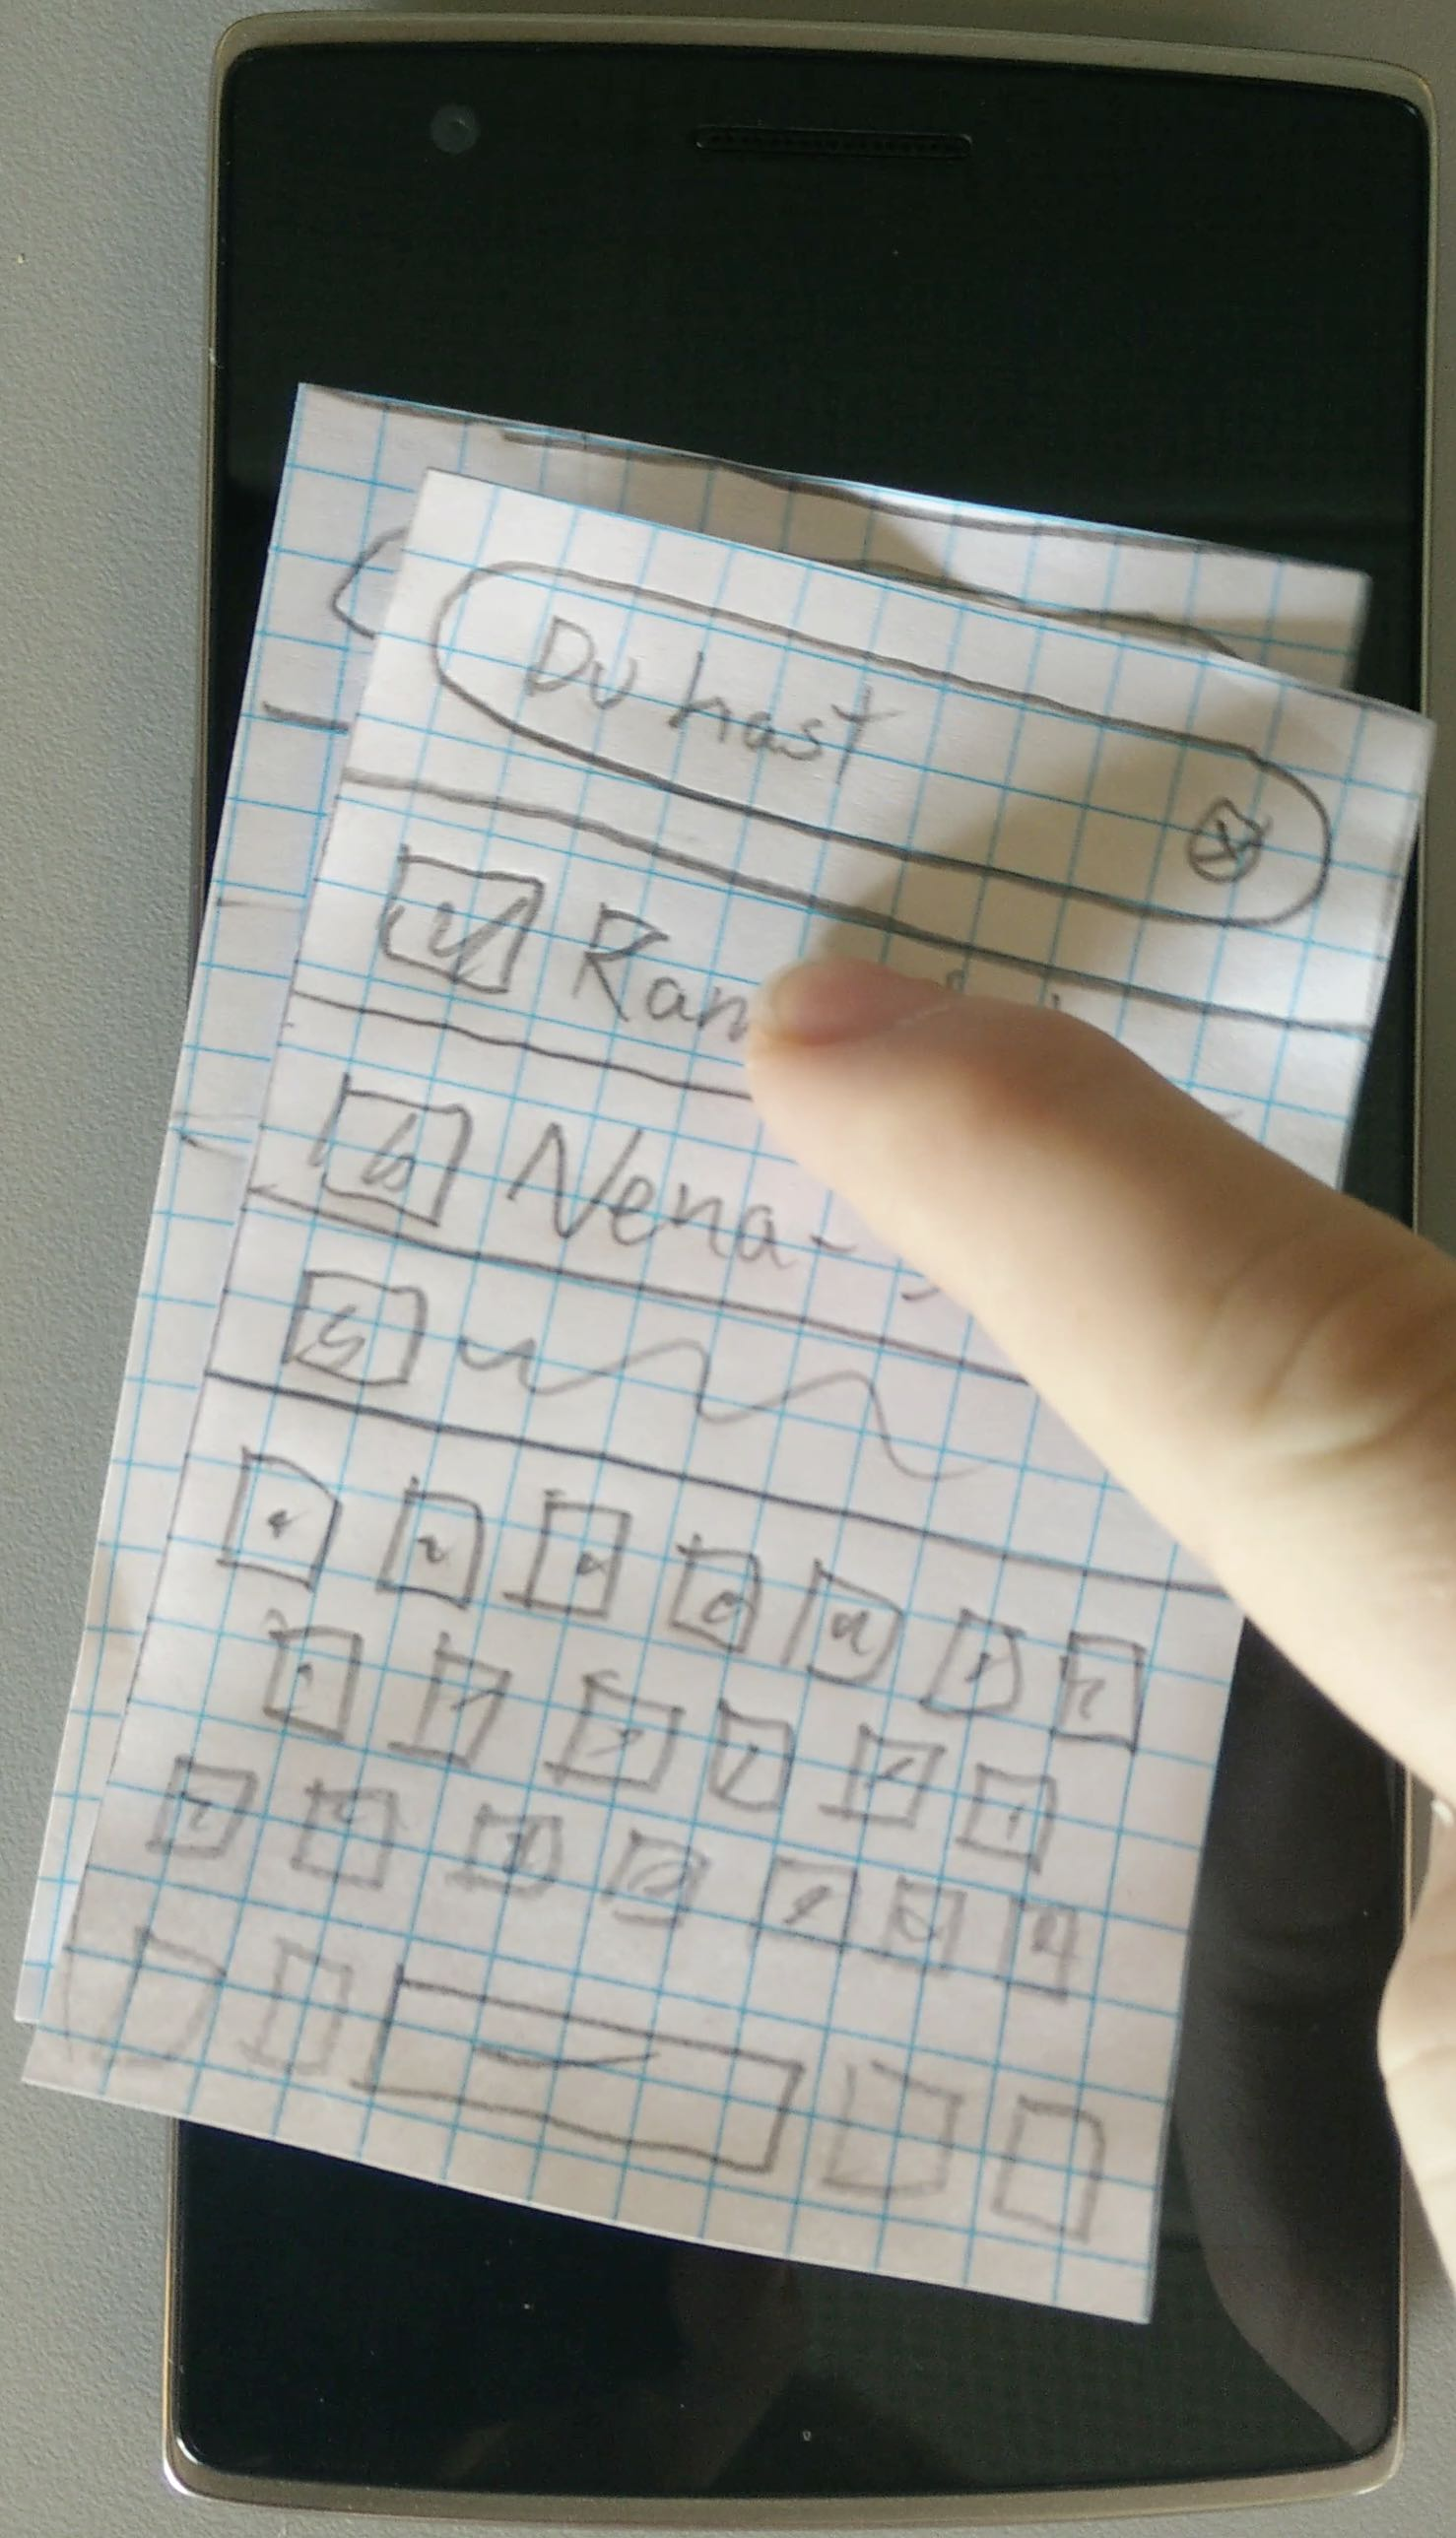
\includegraphics[width=0.33\textwidth]{paperPrototypeAddTrackInteraction}
    \label{fig:paper_prototype_add_track_interaction}
                  }
  \subfloat[Main screen showing the requested track and its position
  on the playlist.]{
    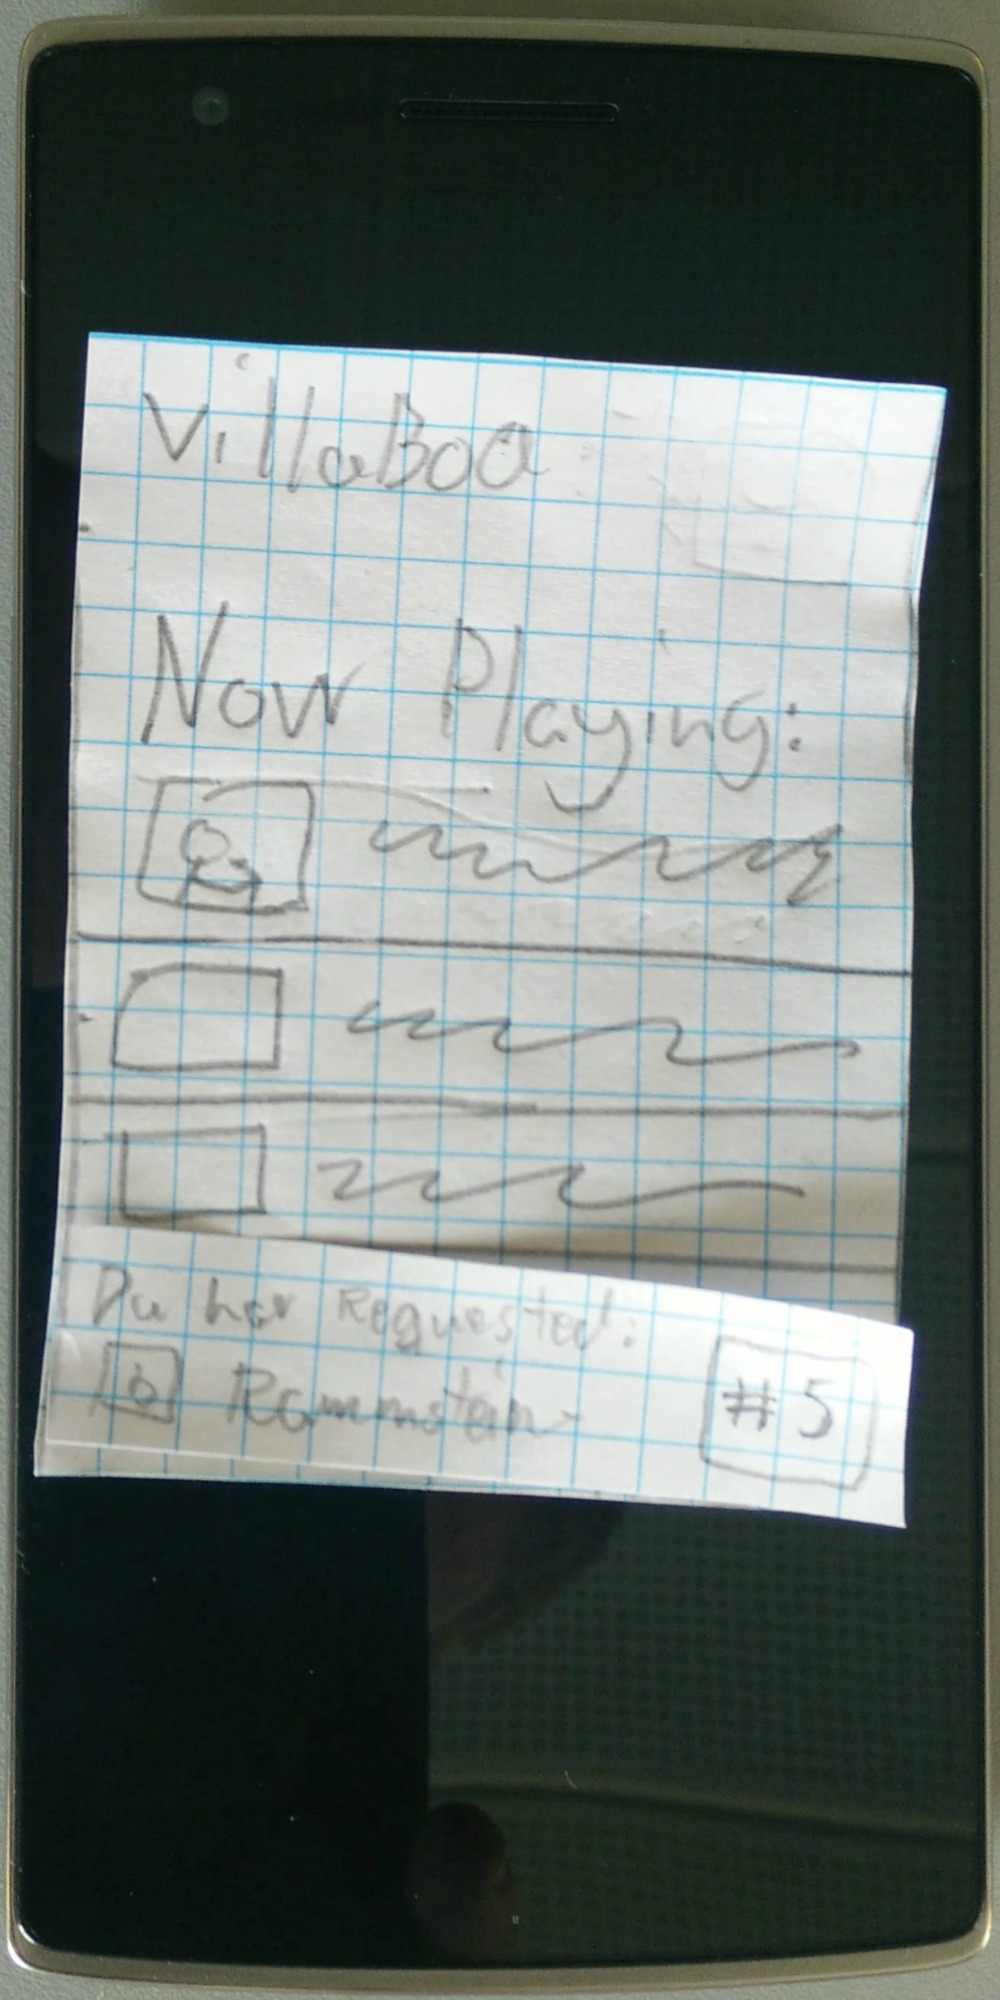
\includegraphics[width=0.33\textwidth]{paperPrototypeAddTrackFeedback}
    \label{fig:paper_prototype_add_track_feedback}
                  }
  \caption{Adding a track onto the playlist.}
\end{figure}

If a track is not present on the playlist, it can be added in the
request screen as shown in
\cref{fig:paper_prototype_add_track,fig:paper_prototype_add_track_interaction,fig:paper_prototype_add_track_feedback}.